\documentclass[addpoints]{exam}

\usepackage{graphbox}
\usepackage{hyperref}
\usepackage{listings}
\usepackage{subcaption}
\usepackage{tabularx}
\usepackage{tikz}
\usetikzlibrary{positioning}

% Header and footer.
\pagestyle{headandfoot}
\runningheadrule
\runningfootrule
\runningheader{CS 440}{HW 3: Meshes and Transformations}{Fall 2022}
\runningfooter{}{Page \thepage\ of \numpages}{}
\firstpageheader{}{}{}

% \qformat{{\large\bf \thequestion. \thequestiontitle}\hfill[\totalpoints\ points]}
\qformat{{\large\bf \thequestion. \thequestiontitle}\hfill}
\boxedpoints

\title{Homework 3: Meshes and Transformations}
\author{CS 440 Computer Graphics\\Habib University}
\date{Fall 2022}

\begin{document}
\maketitle

Each problem below specifies the names of the files that you have to submit for it. Please make sure that your submitted files have the indicated names. Any files in your GitHub repository with these names at the time of the deadline will be considered your submission.

Feel free to make use of the utility files from \href{https://bit.ly/3Bqt8XG}{the website} of the newer edition of the textbook. Specifically, the files containing ``ES6'' in their names. These supersede similarly named files in the folder in that they are compliant with recent JavaScript (JS) standards which deprecate older features that are, in some cases, now considered insecure. You may copy the files \texttt{MVES6.js} and \texttt{initShadersES6.js} to your repository and include the local files in your HTML or include the files over the web.

GLSL has some helpful syntax and types to support geometric computation. You can read about them in the GLSL section toward the bottom of \href{https://webgl2fundamentals.org/webgl/lessons/webgl-shaders-and-glsl.html}{this page}.

\begin{questions}

  \titledquestion{A repository of models}

  \begin{tabularx}{\linewidth}{lX}
    \raisebox{-.95\totalheight}{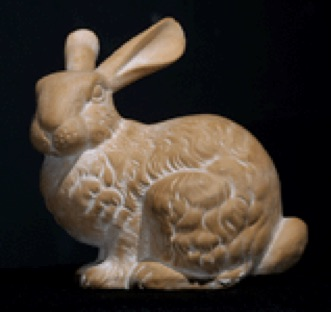
\includegraphics[width=.3\textwidth]{bunny}}
    &
    Browse the \href{http://graphics.stanford.edu/data/3Dscanrep/}{The Stanford 3D Scanning Repository} and download any (or all!) of the 3D models. Write a program to load any of the meshes from file and transform it to WebGL's default clip coordinates such that the aspect ratio of the model is preserved and the model is centered at the origin.
    
Your program's interface should support interaction for the following operations on the loaded model.
\end{tabularx}
  \begin{parts}
    \part Rotate the model slightly about each of the 3 axes in the clockwise or counterclockwise direction.
    \part Shift the model slightly in the positive or negative x, y, or z directions.
    \part Shrink or grow the model slightly along any of the x, y, or z directions.
    \part Reflect the model about any of the axes.
    \part Apply a positive or negative shear to the model along any of the axes.
    \part Reset all transformations.
  \end{parts}

  Take care of the following.
  \begin{itemize}
  \item Make sure to keep the model visible at the end of each operation.
  \item Provide the user the option to specify a local mesh file that contains the model to be loaded.
  \item Use \href{https://registry.khronos.org/OpenGL-Refpages/gl4/html/gl_FragCoord.xhtml}{gl\_FragCoord} or \href{https://registry.khronos.org/OpenGL-Refpages/gl4/html/gl_FragDepth.xhtml}{gl\_FragDepth} to create a perception of depth.
  \end{itemize}
  \underline{Files}: {\tt mesh.html, mesh.js}

\end{questions}

\end{document}

%%% Local Variables:
%%% mode: latex
%%% TeX-master: t
%%% End:
